\section{実験}
\subsection{把持実験}
力覚センサを組み込んだ柔軟指で把持対象物を把持したときのセンサの応答を検証した.実験手順は以下の通りである.把持対象物を\refig{objecht}に示す.計測誤差結果を\refig{result0}に示す.

\begin{enumerate}
  \item 力覚センサを組み込んだ柔軟指で対象物を把持する.  
  \item 把持時の力覚センサの電圧値を測定する.
\end{enumerate}

\subsubsection{引張実験}
引張力を検証することで把持対象物に加わる把持力を測定する.以下に実験手順を示す.
実験で使用したフォースゲージを\refig{force_gauge}に示す.

\begin{enumerate}
  \item 力覚センサを組み込んだ柔軟指で対象物を把持する.  
  \item フォースゲージを用いて対象物を鉛直下向きに引っ張った.
  \item 
\end{enumerate}把持対象物が動いたときの引っ張り力を計測した.

\subsection{結果と考察}

\newpage


%\subsubsection{実験結果}
%使用した指は以下の通りである.実験結果を\reftab{result}にまとめる.把持成功は◯,把持失敗は×を表している.把持対象物Eは上部の突起部と下部の外周部での把持が両方成功した時把持成功とみなした.\reftab{result}の横軸は\refig{denso_parts}の割り振った記号と対応し縦軸は以下の指の番号と対応している.

%\begin{enumerate}
  %\item 柔軟物のない指
  %\item 厚さ3mmのゲルを取り付けた指
  
  
%\end{enumerate}

%\begin{table}[htbp]
 %   \caption{把持実験結果}
 
%  \label{tab::result}
   %\scalebox{3}[1.5]
  % \centering
   %\begin{tabular}{|c||c|c|c|c|c|} \hline
      %    &A    &B     &C      &D     &E        %\\ \hline \hline
 %       (1) & ◯ & ◯  & ×  & ◯ & ×  \\ \hline
   %     (2) & ◯ & ◯  & ◯  & ◯ & ◯  \\ \hline
    %    (3) & ◯ & ◯  & ◯  & ◯ & ◯  \\ \hline
	%	(4) & ◯ & ◯  & ◯  & ◯ & ×  \\ \hline
	%	(5) & ◯ & ◯  & ◯  & ◯ & ×  \\ \hline				
	%	(6) & ◯ & ◯  & ◯  & ◯ & ×  \\ \hline
	%	(7) & ◯ & ◯  & ◯  & ◯ & ×  \\ \hline
	%	(8) & × & ×  & ×  & × & ×  \\ \hline		
	%	(9) & × & ×  & ×  & × & ×  \\ \hline		
			
		
    %\end{tabular}
%\end{table}

%\begin{figure}[h]
%\centering
%\subfloat[把持対象物A]{\includegraphics[scale=0.4]{../figure/result_a.eps}}
%\hspace{5mm}
%\subfloat[把持対象物B]{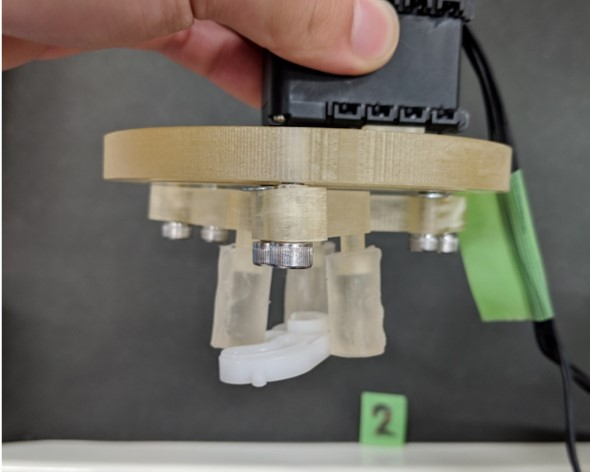
\includegraphics[scale=0.4]{../figure/result_b.eps}}
%\hspace{5mm}
%\subfloat[把持対象物C]{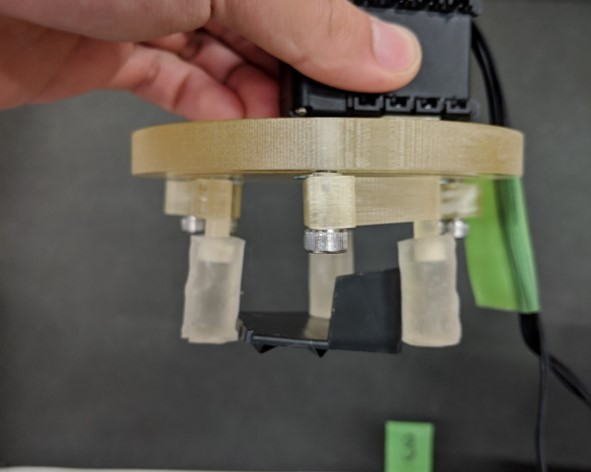
\includegraphics[scale=0.4]{../figure/result_c.eps}}
%\hspace{5mm}
%\subfloat[把持対象物D]{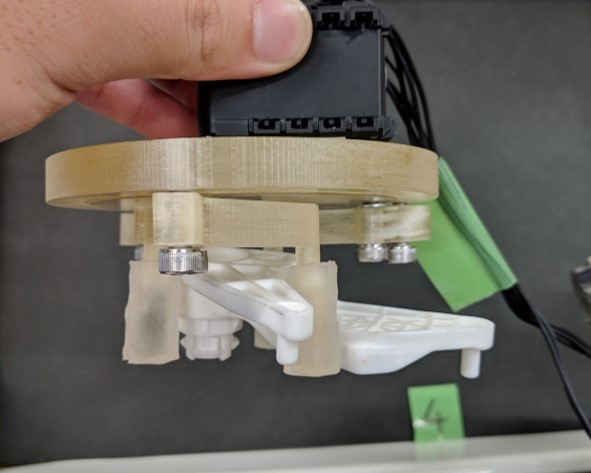
\includegraphics[scale=0.4]{../figure/result_d.eps}}
%\hspace{5mm}
%\subfloat[把持対象物E 上部の突起]{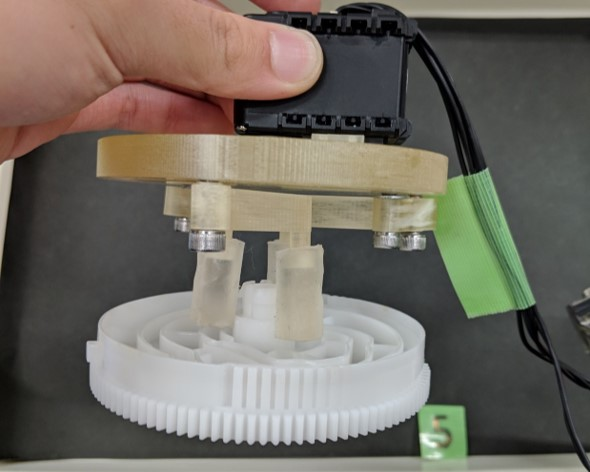
\includegraphics[scale=0.4]{../figure/result_e1.eps}}
%\hspace{5mm}
%\subfloat[把持対象物E 下部の外周部]{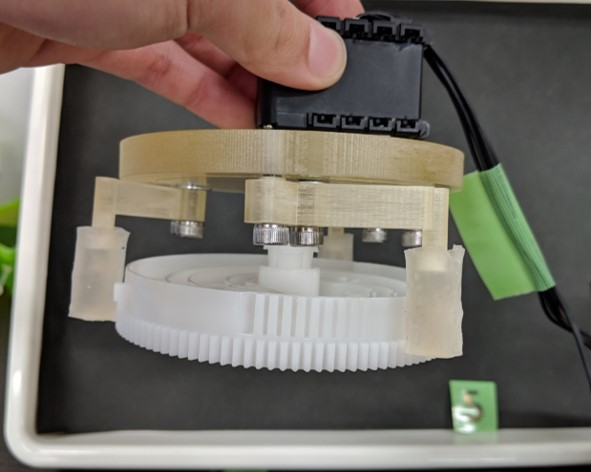
\includegraphics[scale=0.4]{../figure/result_e2.eps}}
%\hspace{5mm}
%\caption{厚さ3mmのゲルの指での把持の様子}
%\label{fig::sisaku}
%\end{figure}


